\chapter{Exercise 06}
\extitle{Ridge Regression}
%******************************************************************************%
%                                                                              %
%                                 Interlude                                    %
%                         for Machine Learning module                          %
%                                                                              %
%******************************************************************************%

\section*{Interlude - Evaluate}

\begin{figure}[h!]
  \centering
  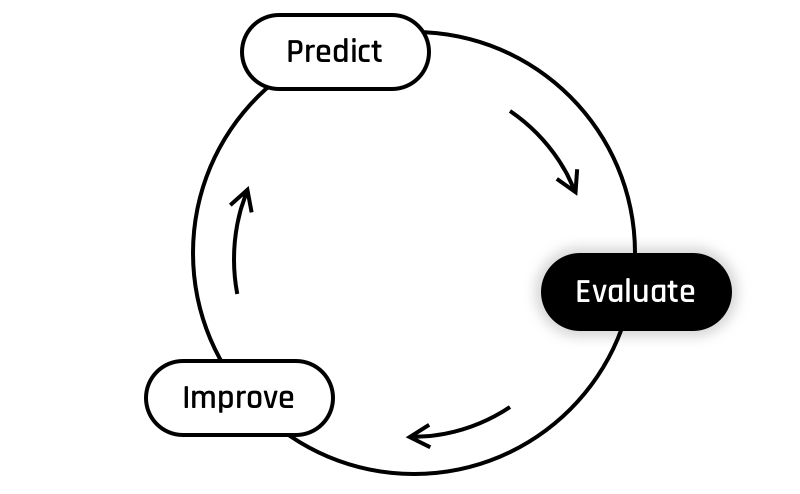
\includegraphics[scale=0.25]{assets/Evaluate.png}
  % \caption{cycle evaluate}
\end{figure}

\subsection*{Introducing the loss function}

How good is our model?  
It is hard to say just by simply looking at the plots!
We can clearly observe that certain regression lines seem to fit the data better than others, but it would be convenient to find a way to measure it. 

\begin{figure}[h!]
  \centering
  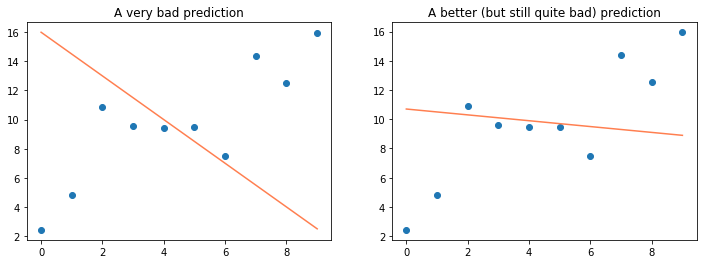
\includegraphics[scale=0.55]{assets/bad_prediction.png}
  \caption{bad prediction}
\end{figure}

To evaluate our model, we are going to use a \textbf{metric} called \textbf{the loss function} (sometimes called \textbf{cost function}).\\
\newline
The loss function tells us how bad our model is performing, how much it \textit{costs} us to use it, how much information we \textit{lose} when we use it.
If the model is good, we won't lose that much; if it's terrible instead, we will have a high loss!

The metric you choose will deeply impact the evaluation (and therefore also the training) of your model.

A frequent way to evaluate the performance of a regression model is to measure the distance between each predicted value ($\hat{y}^{(i)}$) and the real value it tries to predict (${y}^{(i)}$). The distances are then squared, and averaged to get one single metric, denoted $J$:

$$
J(\theta) = \frac{1}{2m}\sum_{i=1}^{m}(\hat{y}^{(i)} - y^{(i)})^2
$$

The smaller, the better! 

\begin{figure}[h!]
  \centering
  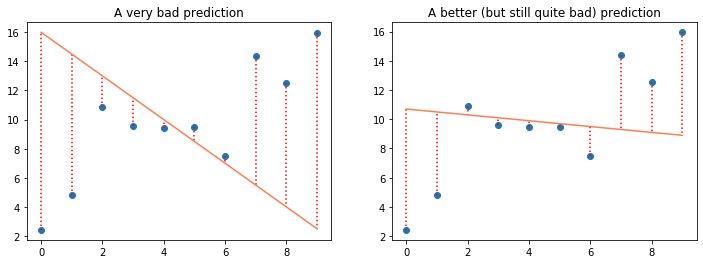
\includegraphics[scale=0.55]{assets/bad_pred_with_distance.png}
  \caption{bad prediction with distance}
\end{figure}

\newpage
\turnindir{ex06}
\exnumber{06}
\exfiles{ridge.py}
\exforbidden{sklearn}
\makeheaderfilesforbidden

% ================================= %
\section*{Objective}
% --------------------------------- %
Now it's time to implement your \texttt{MyRidge} class, similar to
 the class of the same name in \texttt{sklearn.linear\_model}.\\

% ================================= %
\section*{Instructions}
% --------------------------------- %
In the \texttt{ridge.py} file, create the following class as per the instructions given below:\\
\\
\begin{minted}[bgcolor=darcula-back,formatcom=\color{lightgrey},fontsize=\scriptsize]{python}
	class MyRidge(ParentClass):
		"""
		Description:
			My personnal ridge regression class to fit like a boss.
		"""
		def __init__(self,  thetas, alpha=0.001, max_iter=1000, lambda_=0.5):
			self.alpha = alpha
			self.max_iter = max_iter
			self.thetas = thetas
			self.lambda_ = lambda_
			... Your code here ...
	
		... other methods ...
	\end{minted}
\\
Your \texttt{MyRidge} class will have at least the following methods:
\begin{itemize}
  \item \texttt{\_\_init\_\_}, special method, similar to the one you 
  wrote in \texttt{MyLinearRegression} (module06)
  \item \texttt{get\_params\_}, which gets the parameters of the estimator
  \item \texttt{set\_params\_}, which sets the parameters of the estimator
  \item \texttt{loss\_}, which returns the loss between 2 vectors (numpy arrays)
  \item \texttt{loss\_elem\_}, which returns a vector corresponding to the squared 
  diffrence between 2 vectors (numpy arrays)  
  \item \texttt{predict\_}, which generates predictions using a linear model
  \item \texttt{gradient\_}, which calculates the vectorized regularized gradient
  \item \texttt{fit\_}, which fits Ridge regression model to a training dataset
\end{itemize}

\hint{You should consider inheritance from \texttt{MyLinearRegression}.}
\noindent{If \texttt{MyRidge} inheritates from \texttt{MyLinearRegression}, you may not 
need to reimplement the \texttt{predict\_} method.}\\
\\
The difference between the \texttt{MyRidge}'s implementations of \texttt{loss\_elem\_}, \texttt{loss\_}, \texttt{gradient\_} and 
\texttt{fit\_} and the ones in your \texttt{MyLinearRegression} class 
(implemented in module 02) is the use of a regularization term.\\
\hint{
  again, this is a good use case for decorators...
}